%! TeX program = lualatex
%---------------------------ALLGEMEINE IMPORTS-------------------------------------
\documentclass[12pt,english,ngerman]{scrartcl}

\input{./protokoll_template/template.latex/input/shared_preamble.tex}

    % Kopfzeile
\ihead{WS22\\11.11.2022}
\chead{\textsc{Stark} Matthias - 12004907 \\ \textsc{Philipp} Maximilian - 11839611}
\ohead{FLAB 1 \\ Zählrohr}
    % Fußzeile

\begin{document}
%\includepdf{}
\tableofcontents
\newpage

\section{Aufgabenstellung\label{Auf}}



\begin{itemize}
    \item Messung der $\alpha$, $\beta$ und $\gamma$ Strahlung ohne und mit verschiedenen dicken Abschirmungen
    \item Aufnahme der Zählrohrcharakteristik
    \item Aufnahme der Zählstatistik
    \item Bestätigung des Abstandsgesetzes
    \item Bestimmung der Endpunktsenergie über Absorbtion in Aluminium
    \item Aufnahme des Energiespektrums von $\beta$ Strahlung mit Magnetspektrometer
    \item Aufnahme und Kalibrierung des $\gamma$ Spektrums
    \item Aufnahme des komplexen $\gamma$ Spektrums und seinen Zerfallsprodukten
\end{itemize}

\section{Grundlagen}\label{Grund}


\section{Versuchsanordnung}\label{sec:Versuchsanordnung}

Im Laufe des Versuchs wurden 3 verschiedene Aufbauten verwendet die im Verlauf modifiziert wurden.

\subsection{Digitalzähler}\label{aufbau_Digz}

Für den ersten Teil des Versuchs wird folgender Versuchsaufbau aus \autoref{fig:digz} realisiert.
Dabei wird das Präparat in die dafür vorgesehene Halterung geschoben, hinter der sich das Zählrohr befindet, 
welches mit dem Digitalzähler verbunden ist, wodurch ein einfaches Ablesen der Counts ermöglicht wird.
Auf der optischen Bank kann der Abstand zwischen Präparat und Zählrohr variiert und abgelesen werden.
Dabei ist zu beachten, dass die abgelesene Distanz auf der optischen Bank nicht dem tatsächlichen Abstand zwischen 
Probe und Zählrohr entspricht, da sich diese nicht direkt über den Sockel befinden. Um im späteren Verlauf des Versuchs die 
Aluminiumbleche zu befestigen, wird die entsprechende Halterung auf die optische Bank gesteckt.

\begin{figure}[H]
  \begin{center}
  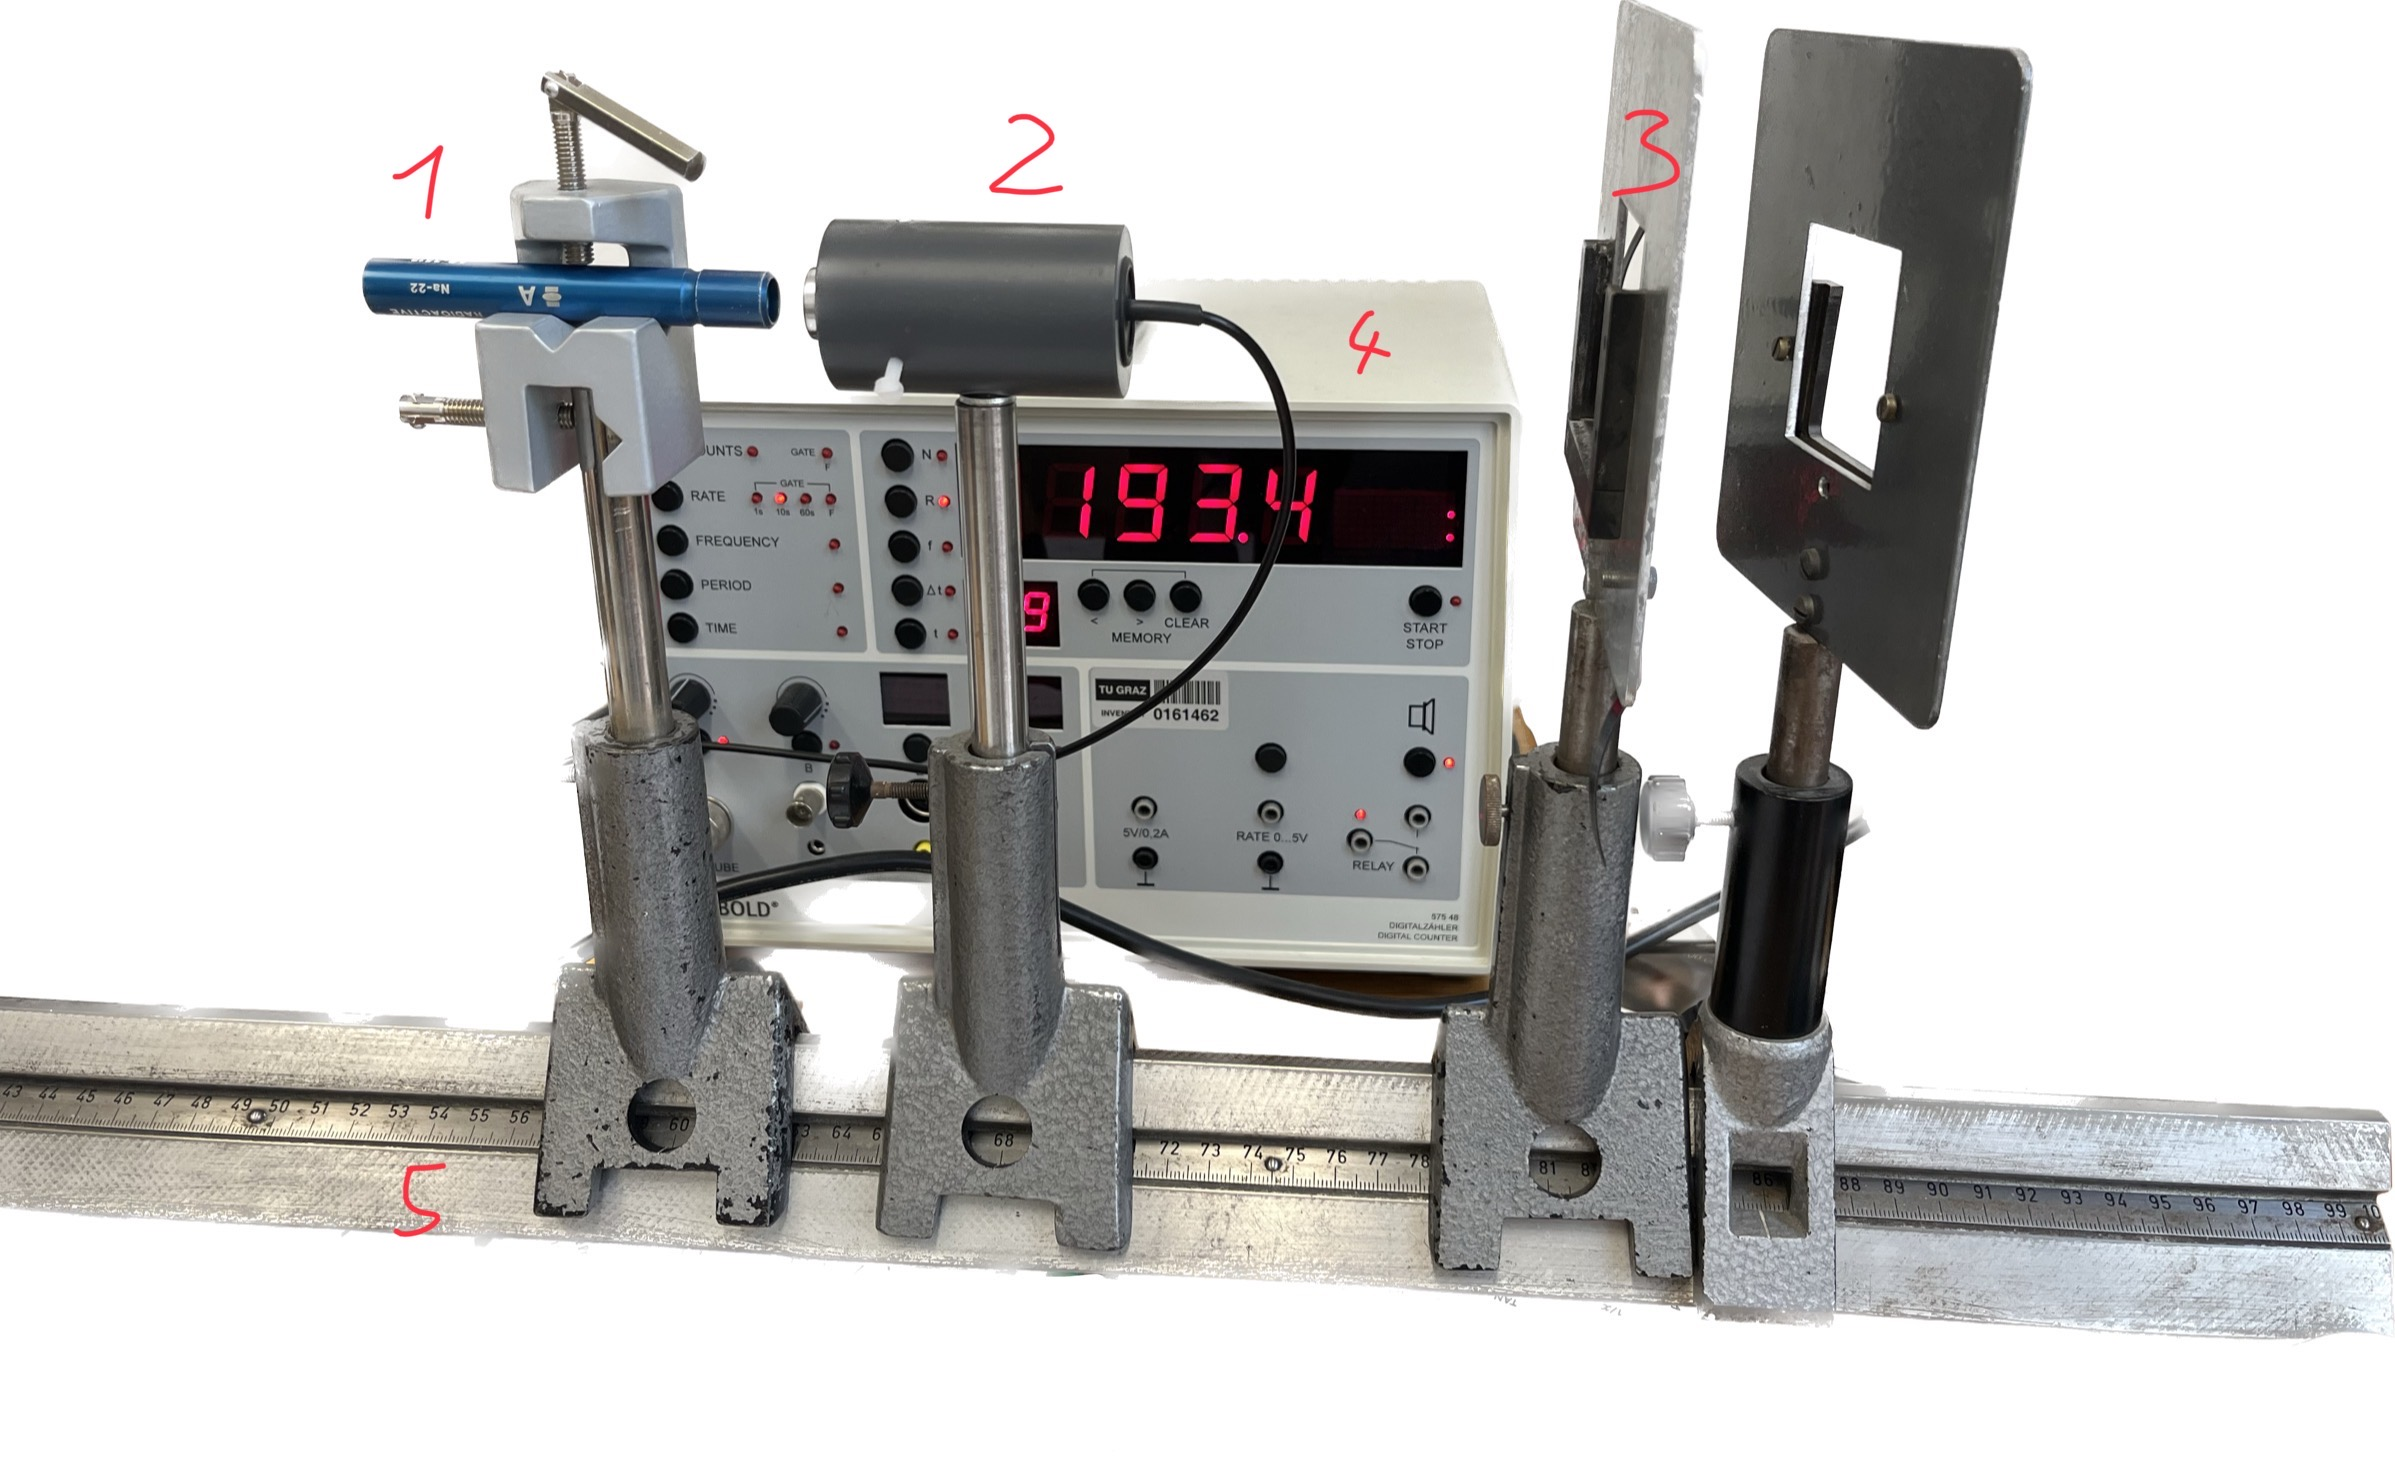
\includegraphics[width=0.8\textwidth]{./figures/digz.png}
	\end{center}
	\caption[Aufbau des Digitalzähler]{Aufbau des Digitalzähler \\ 1 $\dots$ Halterung für radioaktive Quelle\\ 2 $\dots$ Zählrohr 
    \\3 $\dots$ Halterung um später das Aluminium zu Befestigen \\ 4 $\dots$ Digitalzähler 
    \\ 5 $\dots$ optische Bank um den Abstand zu variieren}
	\label{fig:digz}
    
\end{figure}

\subsection{Magnetfeldspektrometer}\label{sec:aufbau_Magnetfeldspektrometer}

Um $\beta$ Strahlung messbar zu machen, wird folgender Aufbau aus \autoref{fig:mag} verwendet. 
Dabei wird das radioaktive Präparat in das dafür vorgesehene Loch gesteckt. Durch die Spule 
wird ein Magnetfelds erzeugt, wodurch die Betastrahlung aufgrund von Lorentzkraft abgelenkt wird,
weshalb die Hallsonde auch schräg zur Quelle angeordnet ist. Dies stellt sicher, dass keine 
Gammastrahlung gemessen wird. Die Stärke des Magnetfelds wird durch das Netzgerät bestimmt.


\begin{figure}[H]
    \begin{center}
    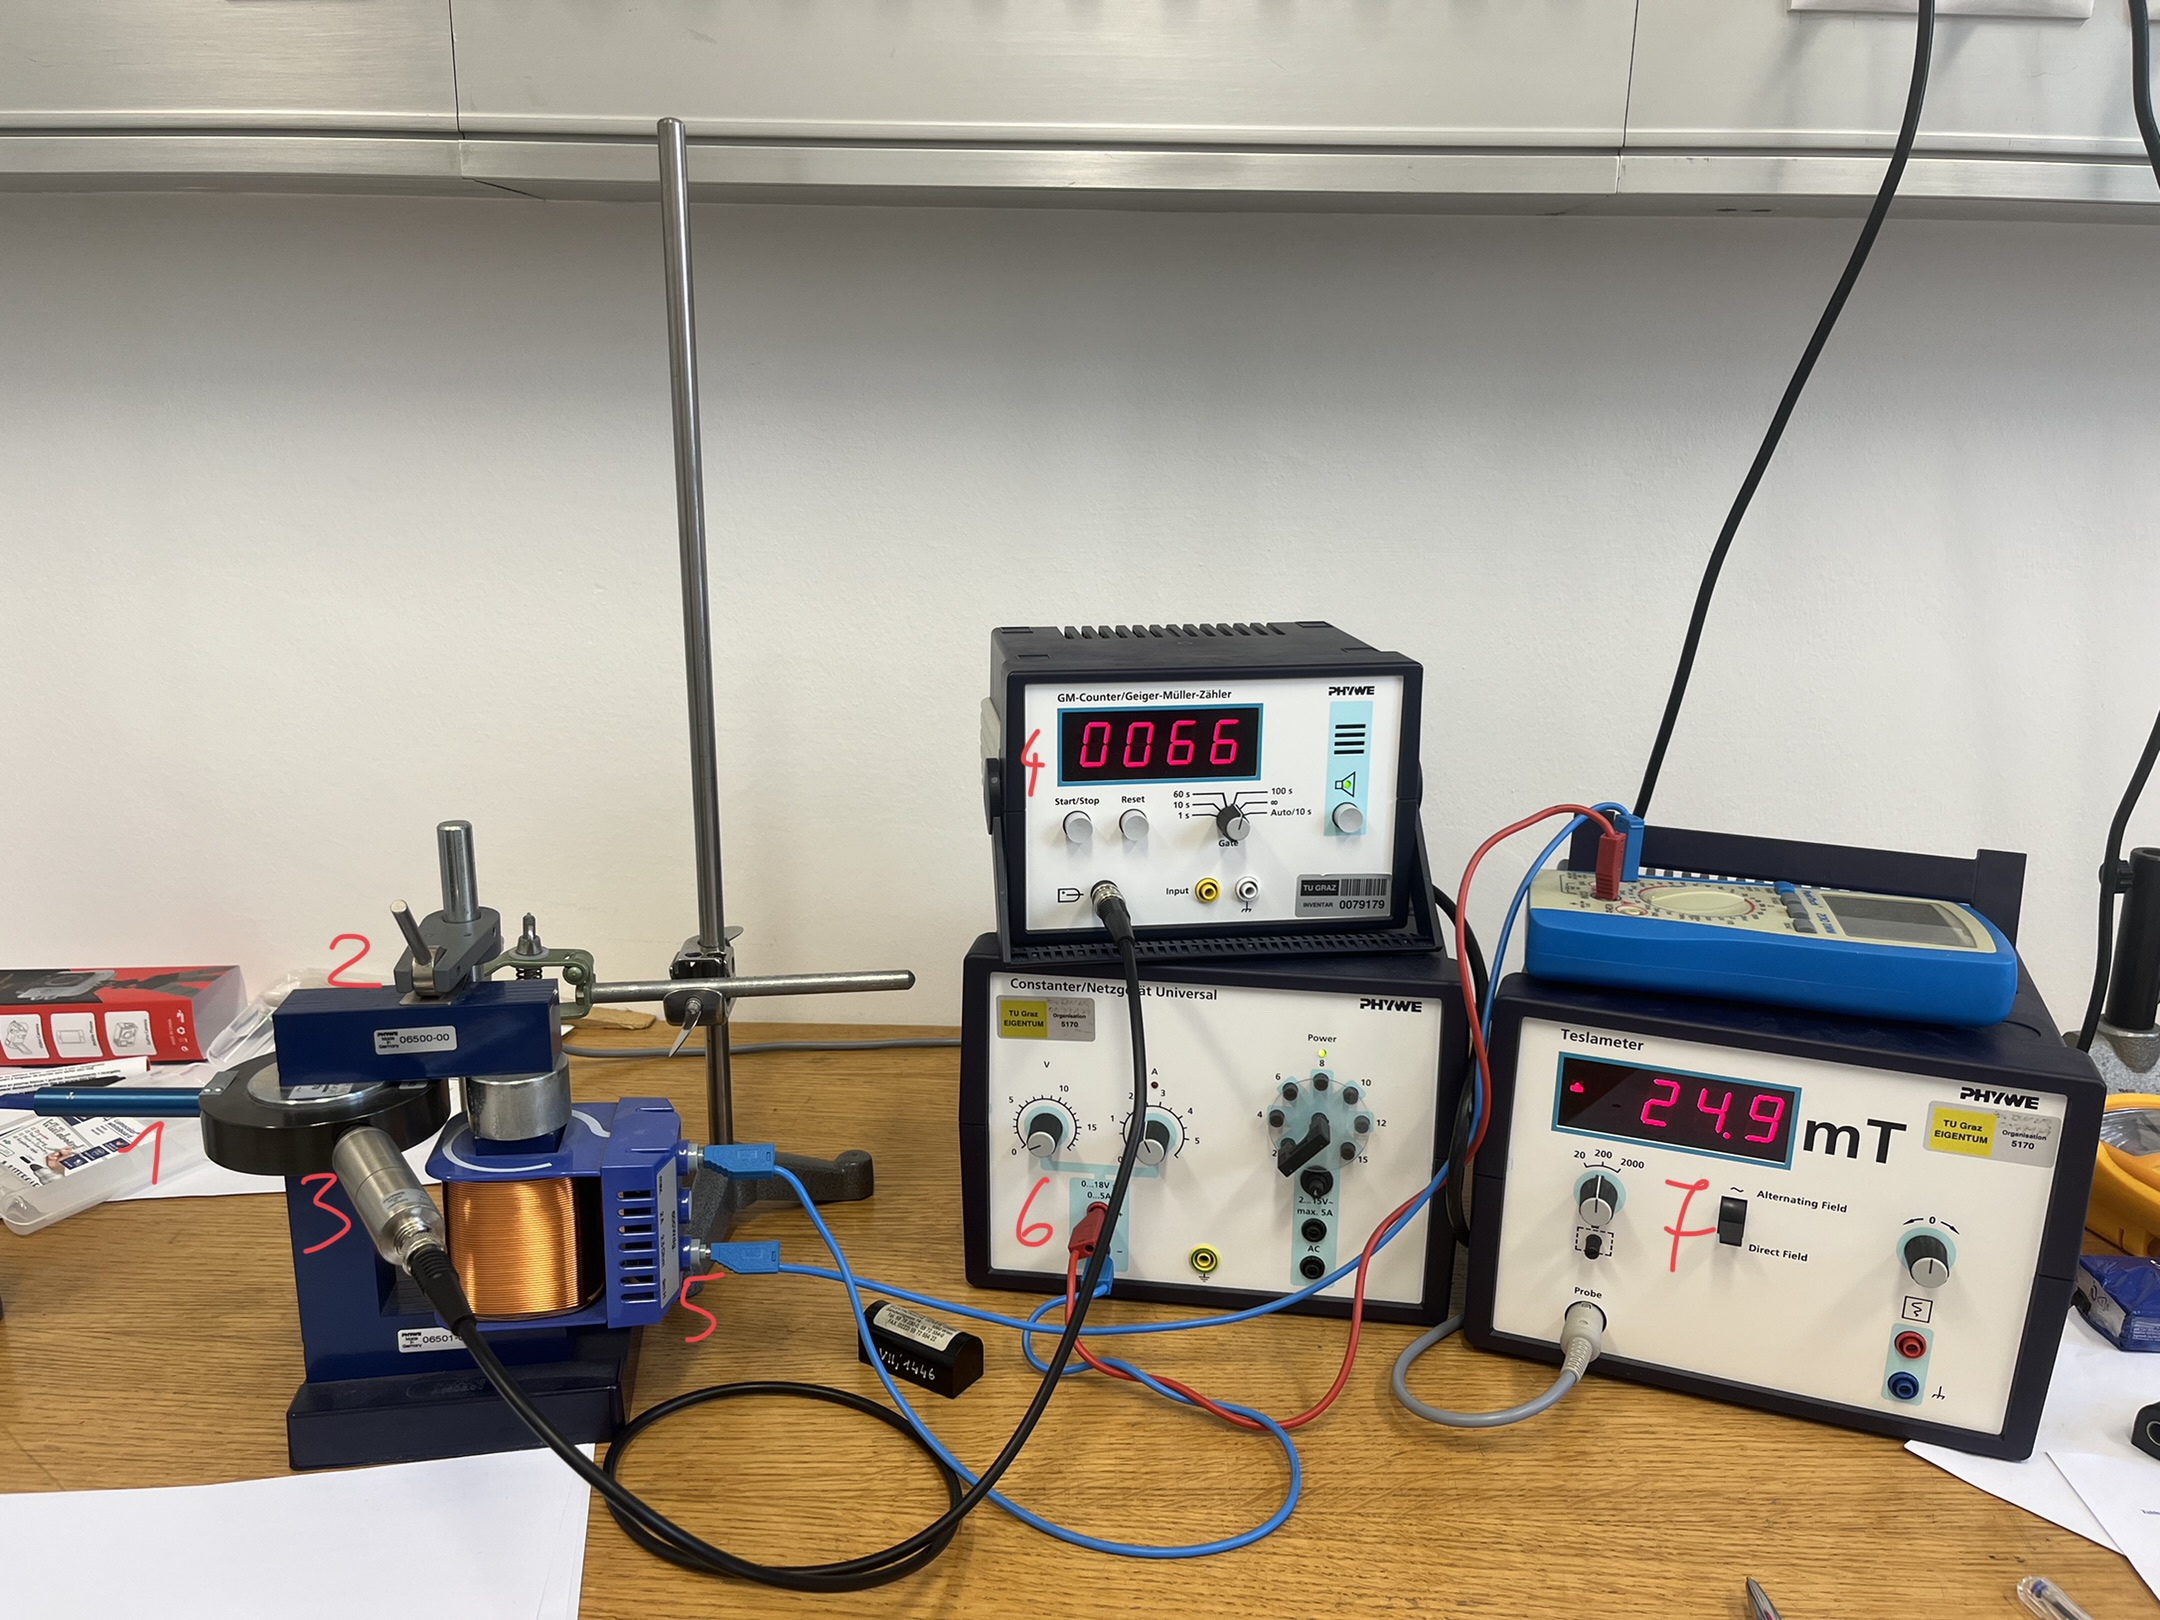
\includegraphics[width=0.8\textwidth]{./figures/mag_new.png}
      \end{center}
      \caption[Aufbau des Magnetfeldspektrometers]{Aufbau des Magnetfeldspektrometers \\ 1 $\dots$ Radioaktive Quelle\\ 2 $\dots$ Hallsonde (nicht sichtbar im Foto) 
      \\3 $\dots$ Epfänger des Geiger-Müller-Zählers \\ 4 $\dots$ Anzeige des Geiger-Müller-Zählers
      \\5 $\dots$ Spule um das Magnetfeld zu erzeugen \\ 6 $\dots$ Netzgerät für das Magnetfeld 
      (Stecker um die Polung des Magnetfelds zu Ändern)
    \\7 $\dots$ Teslameter um die Stärke des Magnetfelds zu bestimmen}
      \label{fig:mag}
      
  \end{figure}


\subsection{Szintilationszähler}\label{aufbau_szinti}

Der Aufbau des Szintilationszählers ist in folgender \autoref{fig:szinti} sichtbar. Die radioaktive Quelle wird in die, dafür
vorgesehene, Halterung ober den Szintilationszähler gesteckt. Um eine Auswertung am PC zu ermöglichen, wird ein Cassy-Lab 
als Schnittstelle verwendet.

\begin{figure}[H]
    \begin{center}
    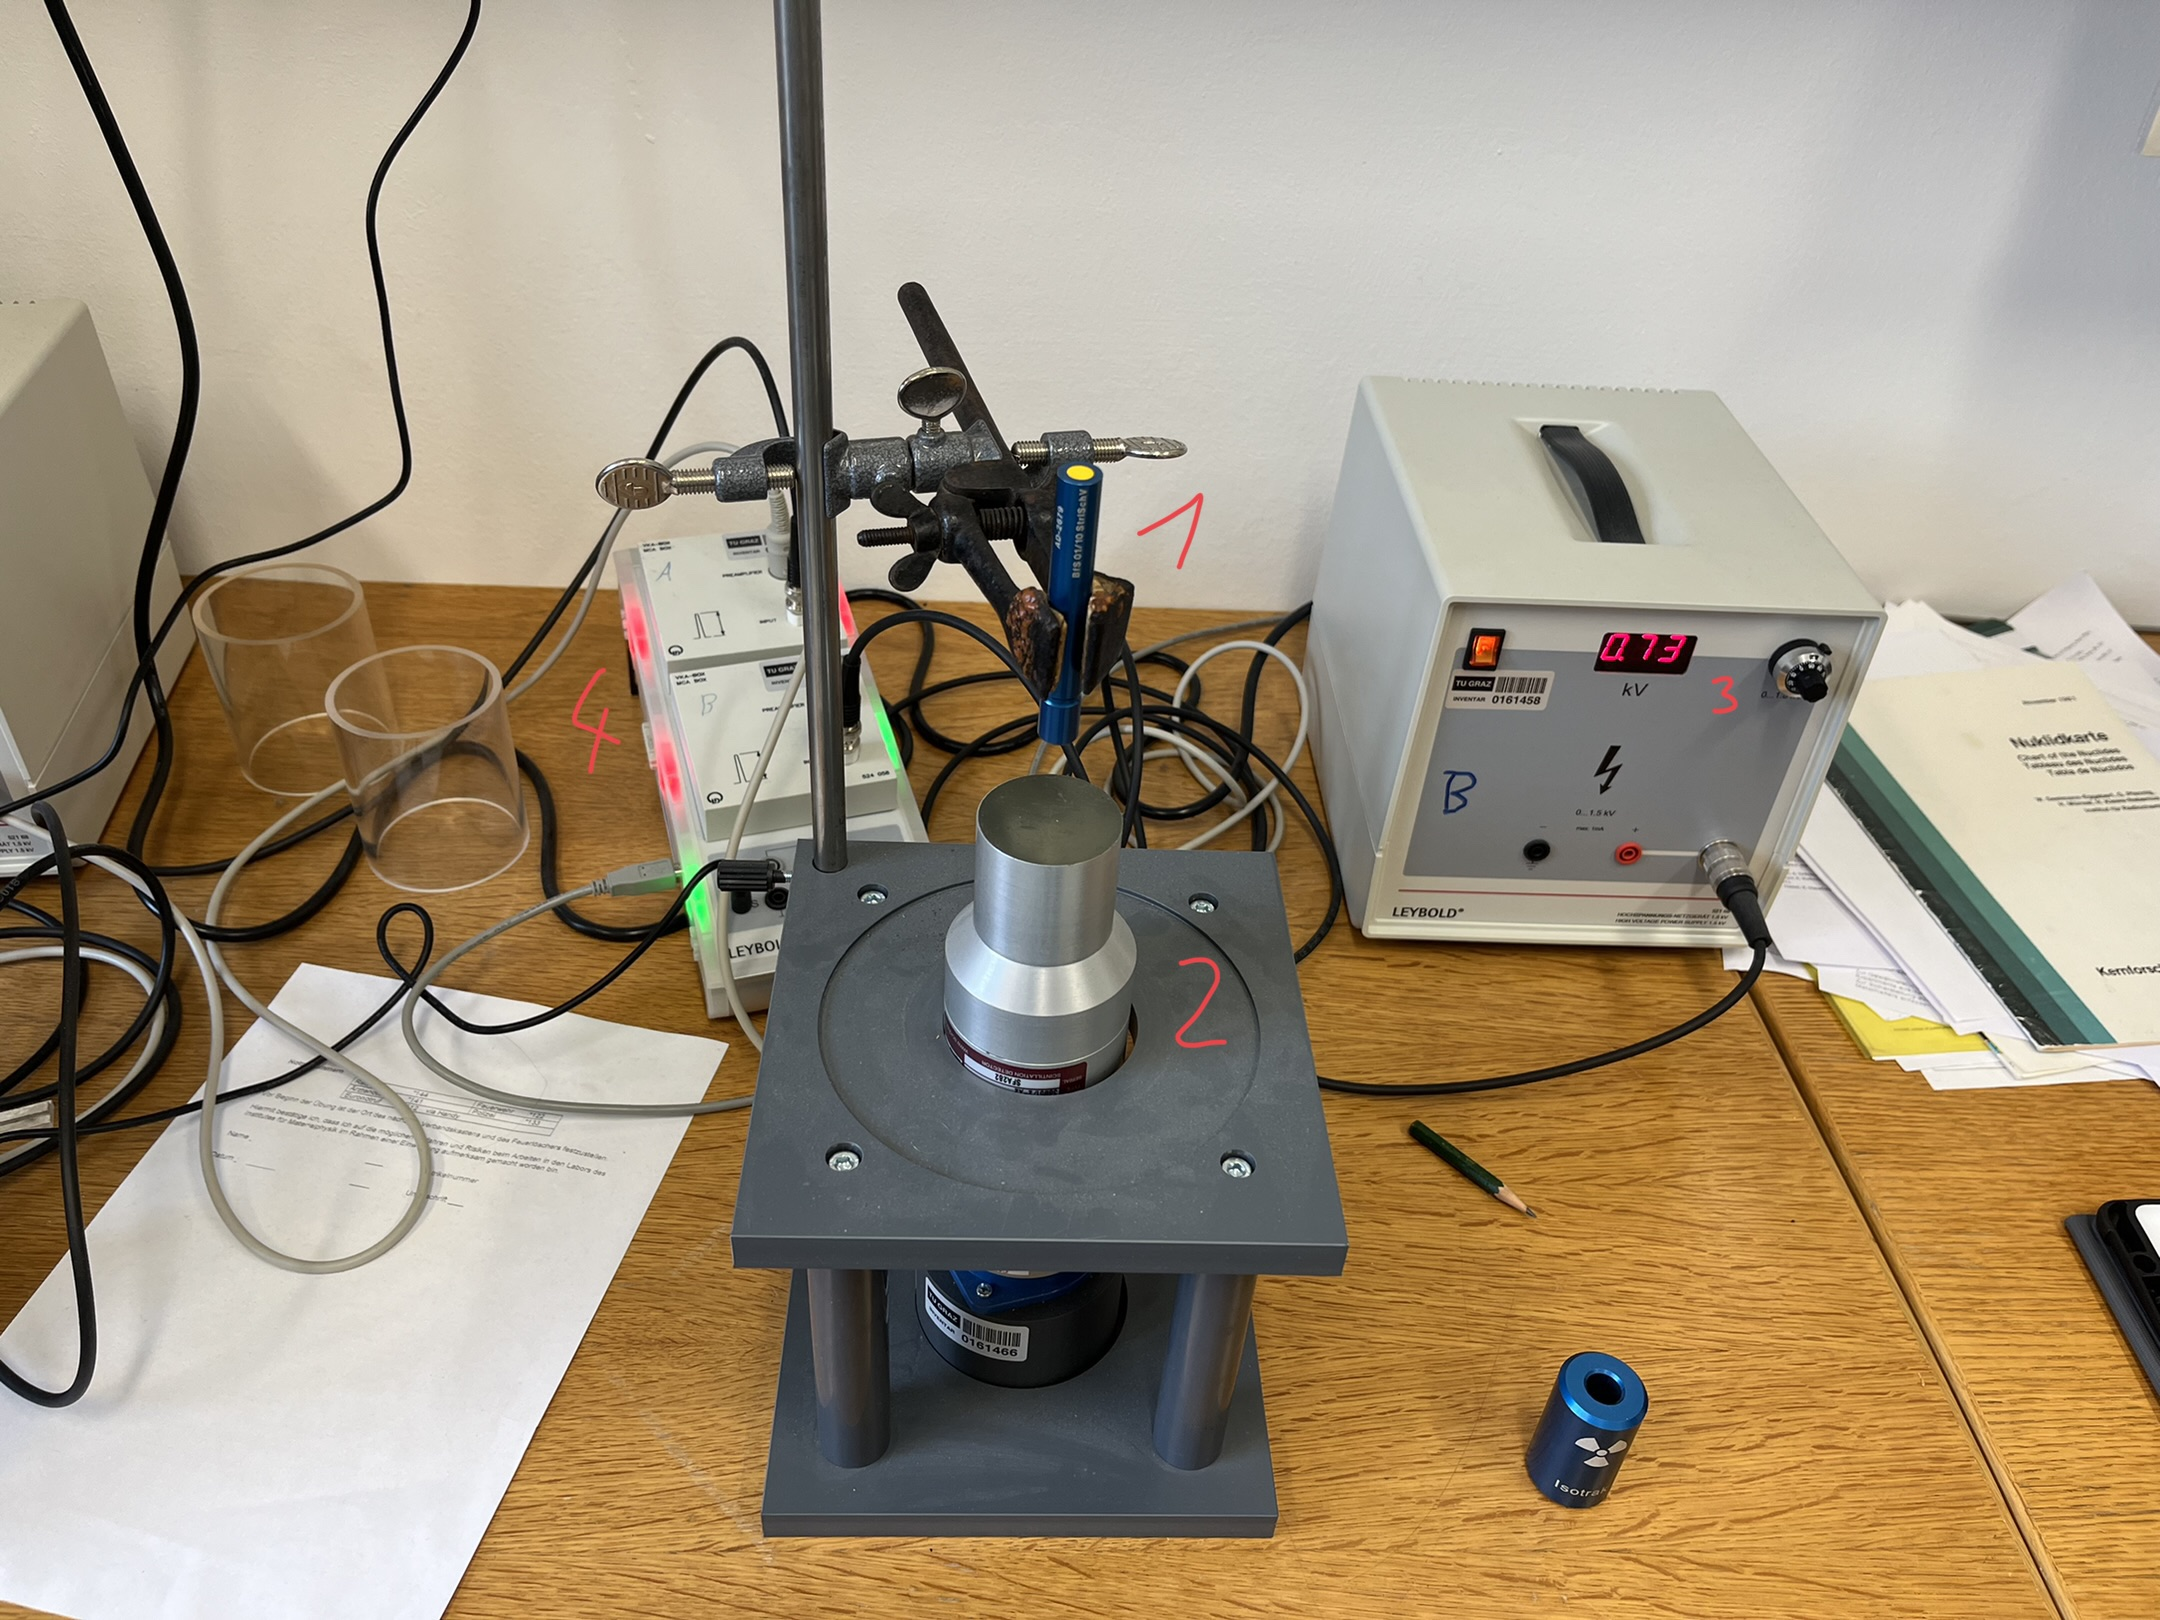
\includegraphics[width=0.8\textwidth]{./figures/szinti.png}
      \end{center}
      \caption[Aufbau des Szintilationszählers]{Aufbau des Szintilationszählers \\ 1 $\dots$ Radioaktive Quelle\\ 2 $\dots$ Szintilationszähler
      \\3 $\dots$ Spannungsgenerator \\ 4 $\dots$ Cassy-Lab um Auswertung am PC zu ermöglichen}
      
      \label{fig:szinti}
      
  \end{figure}


\section{Geräteliste}

%Geräteliste im teachcenter

\section{Versuchsdurchführung \& Messergebnisse}\label{sec:Durchfuhrung}

\subsection{Messung der \texorpdfstring{$\alpha$}{alpha}, \texorpdfstring{$\beta$}{beta} und \texorpdfstring{$\gamma$}{gamma} Strahlung ohne und mit verschiedenen dicken Abschirmungen}

Um die Abschirmung Strahlungen zu Messen, wir der Versuchsaufbau, wie in \autoref{aufbau_Digz} beschrieben, vorgenommen. 
Die Torzeit am Digitalzähler wird dabei auf \SI{10}{\second} gestellt. Als radioaktive Quelle wird \ch{^{22}_{11}Na} verwendet, welche, wie 
bereits beim Aufbau erklärt, in die dafür vorgesehene Halterung gesteckt wird. Der Abstand zwischen der Quelle und dem Zählrohr
wird dabei so gering gewählt, dass die dickste Abschirmungsprobe problemlos dazwischen gehalten werden kann, ohne gegen
die Probe oder das Zählrohr zu stoßen. Diese Distanz zwischen der radioaktiven Quelle und dem Zählrohr wird mit einem Lineal
vermessen und beträgt \SI{15(2)}{\mm}. Die unterschiedlichen Abschirmungen werden der Reihe nach in den Aufbau gehalten und die 
entsprechenden Zählraten notiert, was in folgender \autoref{tab:abschirmung} sichtbar ist. Dabei ist zu Beachten, dass die 
jeweilige Abschirmung die gesamte Torzeit im Aufbau ist und man damit nicht gegen die Probe oder das Zählrohr stößt.

%tab einfügen (von zettel)
%\label{tab:abschirmung}

\subsection{Aufnahme der Zählrohrcharakteristik}

Um die Zählrohrcharakteristik zu bestimmen wird der Aufbau aus \autoref{aufbau_Digz} realisiert.
Als radioaktive Quelle wird erneut \ch{^{22}_{11}Na} in die dafür vorgesehene Halterung gesteckt. Nun wird die Betriebsspannung des
Netzgerätes so lange gesenkt, bis durch den Digitalzähler kein Geräusch hörbar ist, was anzeigt, dass keine Strahlung auf das 
Zählrohr gelangt, was bei \SI{316}{\volt} der Fall war. Nun wird die Spannung in kontinuierlich erhöht, bis ein Wert von 
\SI{600}{\volt} erreicht ist und die entsprechenden Counts
notiert, was in folgender \autoref{tab:zaelrohrchar} sichtbar ist.

%\label{tab:zaelrohrchar}


\subsection{Aufnahme der Zählstatistik}

Um die Zählstatistik durchzuführen wird erneut der Versuchsaufbau aus \autoref{aufbau_Digz} verwirklicht. Auch wird erneut
\ch{^{22}_{11}Na} als radioaktive Quelle verwendet.
Die Torzeit beträgt für diesen Teil des Versuchs \SI{1}{\second}. Wegen der großen Datenmenge werden die erhaltenen Counts über den
Memory Speicher des Digitalzählers direkt auf den Computer übertragen. Die erhaltenen Ergebnisse sind in folgender 
\autoref{tab:zahlstatistik} aufgelistet.


%Daten von Brossman auf Stick
%\label{tab:zahlstatistik}


\subsection{Bestätigung des Abstandsgesetzes}

Um das Abstandsgesetz zu Bestätigen wird erneut der Versuchsaufbau aus \autoref{aufbau_Digz} verwendet. Um die verschiedenen 
Abstände zu ermöglichen, wird die radioaktive Quelle, erneut \ch{^{22}_{11}Na}, vom Zählrohr entfernt und die entsprechenden Counts bei
einer Torzeit von \SI{10}{\second} in \autoref{tab:abstandsgesetz} vermerkt. Bei der Abstandsbestimmung ist zu beachten,
dass der tatsächliche Abstand zwischen Quelle und Zählrohr vermerkt wird und nicht jener auf der optischen Bank. Um allerdings
den Abstand zu erhöhen kann auf die Skala der optischen Bank geachtet werden, da es sich um eine Differenzmessung handelt 
und so ausgeschlossen werden kann, dass sich die entstehenden Unsicherheiten durch die Messung mittels Lineal gegenläufig auswirken.


%\label{abstandsgesetz}

\subsection{Bestimmung der Endpunktsenergie über Absorbtion in Aluminium}

Um die Endpunktsenergie zu Bestimmen, wird erneut der Versuchsaufbau aus \autoref{aufbau_Digz} verwendet. Um die unterschiedlichen
Aluminiumdicken zu realisieren, werden verschieden Dias mit unterschiedlicher Anzahl an Aluminiumfolien in die dafür vorgesehene
Halterung geschoben. Als radioaktive Quelle wird erneut \ch{^{22}_{11}Na}, sowie eine Torzeit von \SI{10}{\second} verwendet. Die abgelesenen 
Werte sind in folgender \autoref{tab:alu} festgehalten.

%todo \label{tab:alu}

\subsection{Aufnahme des Energiespektrums von \texorpdfstring{$\beta$}{beta} Strahlung mit Magnetspektrometer}

Um das Energiespektrum der $\beta$ Strahlung zu bestimmen wird der Aufbau aus \autoref{sec:aufbau_Magnetfeldspektrometer} realisiert.
Als radioaktive Quelle wird erneut \ch{^{22}_{11}Na} in die dafür vorgesehene Halterung gesteckt. Nun wird die Betriebsspannung des
Netzgerätes so lange gesenkt, bis das erzeugte Magnetfeld in etwa \SI{5}{\milli\tesla} entspricht. Bei den Anschlüssen der 
Spule ist dabei zu beachten, dass das Magnetfeld richtig gepolt ist, um die Strahlung
in die richtige Richtung abzulenken. Nun wird die Spannung durch betätigen des entsprechenden Rades kontinuierlich erhöht
und die jeweiligen Zerfälle bei einer Torzeit von \SI{100}{\second} gemeinsam mit dem jeweiligen Wert des Magnetfelds in folgender
\autoref{tab:magnetspektrometer} aufgelistet. Dabei ist auch wichtig, dass die Hintergrundstrahlung im entsprechenden Gebäude
gemessen wird, indem die selbe Messung auch einmal ohne eingelegte radioaktive Quelle durchgeführt wird. Der dabei erhaltenen
Wert muss dann von den vorherigen Werten abgezogen werden.

%todo \label{tab:magnetspektrometer}

\subsection{Aufnahme und Kalibrierung des \texorpdfstring{$\gamma$}{gamma} Spektrums}

Um das $\gamma$ Spektrum zu kalibrieren wird der Versuch wie in \autoref{aufbau_szinti} erklärt aufgebaut. Um das
Referenzspektum aufzunehmen wird eine \ch{^{137}_{55}Cs} Quelle in die Halterung
eingesetzt. Für die Hochspannung wird dabei ein Wert von \SI{0.73}{\kilo\volt} eingestellt.
%todo Chemie
Mithilfe des Chassy-Labs werden die erhaltenen Daten direkt an den Computer gesendet, wodurch die entsprechenden Spektren geplottet
werden können. Da hier die Werte für die Peaks bekannt sind, kann so eine Kalibrierungskurve erzeugt werden, was in folgender 
\autoref{abb:kalibrierung} sichtbar ist.

%todo \label{abb:kalibrierung}


\subsection{Aufnahme des komplexen \texorpdfstring{$\gamma$}{gamma} Spektrums und seinen Zerfallsprodukten}

Der Versuch wird die zuvor beschrieben wie in \autoref{aufbau_szinti} aufgebaut, auch wird erneut eine Spannung von \SI{0.73}{\kilo\volt}
verwendet. Als radioaktive Quelle wird für diesen Teil des Versuchs das zu vermessende Ra-226 verwendet. auch diese Werte werden 
auf den Computer übertragen und den zuvor erzeugten Plot bei einer Laufzeit von \SI{2400}{\second} beigefügt. Anhand des zuvor
bestimmten Referenzspektums können nun die Peaks des Ra-226 Spektrums vermessen werden.

%todo chemie




\section{Auswertung}\label{sec:Auswertung}

\subsection{Messung der \texorpdfstring{$\alpha$}{alpha}, \texorpdfstring{$\beta$}{beta} und \texorpdfstring{$\gamma$}{gamma} Strahlung ohne und mit verschiedenen dicken Abschirmungen}



\subsection{Aufnahme der Zählrohrcharakteristik}




\subsection{Aufnahme der Zählstatistik}


\subsection{Bestätigung des Abstandsgesetzes}


\subsection{Bestimmung der Endpunktsenergie über Absorbtion in Aluminium}


\subsection{Aufnahme des Energiespektrums von \texorpdfstring{$\beta$}{beta} Strahlung mit Magnetspektrometer}


\subsection{Aufnahme und Kalibrierung des \texorpdfstring{$\gamma$}{gamma} Spektrums}


\subsection{Aufnahme des komplexen \texorpdfstring{$\gamma$}{gamma} Spektrums und seinen Zerfallsprodukten}






\section*{Diskussion}\label{sec:diskussion}


%verschieben der Hall sonde bei mag

\section{Zusammenfassung}



\newpage

\printbibliography
\listoffigures
\listoftables
\end{document}
